\documentclass[9pt,twoside,lineno]{pnas-new}
% Use the lineno option to display guide line numbers if required.

\templatetype{pnassupportinginfo}

\title{Water resource utilization regimes at a basin scale: transition framework and development traps}
\author{Shuang Song, Shuai Wang, Bojie Fu, Xutong Wu (complete author list)}
\correspondingauthor{Shuai Wang.\\E-mail: shuaiwang@bnu.edu.cn}

\begin{document}

%% Comment out or remove this line before generating final copy for submission; this will also remove the warning re: "Consecutive odd pages found".
% \instructionspage

\maketitle

%% Adds the main heading for the SI text. Comment out this line if you do not have any supporting information text.
\SItext test


% \subsection*{Brief description of Supplementary Information contents: }
% Type or paste text here. This should be additional explanatory text such as an extended technical description of results, full details of mathematical models, etc.   

% \section*{Supplementary Information Methods}
\section*{Methods S1. Definition of study area}
% 黄河经历了水资源开发利用和制度改革
The study area is the Yellow River Basin (YRB), which has experienced the most intense water exploitation and the most dramatic shifts of management regime (Supplementary Fig. 1). According to ecological zoning, landscapes types, water resource zoning et al., the Yellow River Basin can be divided into four different regions (supplementary Fig. 2), which has been widely recognized (ref.). Using this division, there are also some differences of nature between different regions regarding water utilization regimes (supplementary Fig. 3):
\begin{itemize}
    \item \textbf{Source Region (SR):} Over 50\% of natural runoff was produced in this region. The most ecology function here is water conservation, as sparsely populated and less economically developed.
    \item \textbf{Upper Region (UR):} With the highest per capita irrigated land area, there are numbers of large irrigation lands in this region. However, because of backward production methods, efficiency of irrigation are used to be very low.
    \item \textbf{Middle Region (MR):} Crossing Loess Plateau, famous rich-sand area, Yellow River loads most of its sediments here with the highest soil erosion risk. To reverse this situation, the grain for green project changed the water utilization here strikingly.
    \item \textbf{Lower Region (LR):} With dense population and the traditional agricultural trajectory, lower region used to be the largest water use region. However, as the industrial transformation going, proportion of agriculture keeps decreasing, but LR is still the largest water use region in each aspect.
\end{itemize}

\subsection*{Introduction of Yellow River Basin}
\subsection*{Subarea of Yellow River Basin}
\subsection*{General situation of water use in the YRB}

\section*{Methods S2. Detailed information on dataset and processing}
Since the Yellow River Basin consists of ten provincial areas, the above division can also maintain broad consistency with administrative divisions.
Add a materials' subsection if you need to.

\section*{Methods S3. Water Utilization Regime Index}
Add a methods subsection if you need to.


%%% Each figure should be on its own page
\begin{figure}
    \centering
    
\includegraphics[width=\textwidth]{../../figures/placeholder_s}
    \caption{Yellow River Basin}
\end{figure}


\begin{figure}
\centering
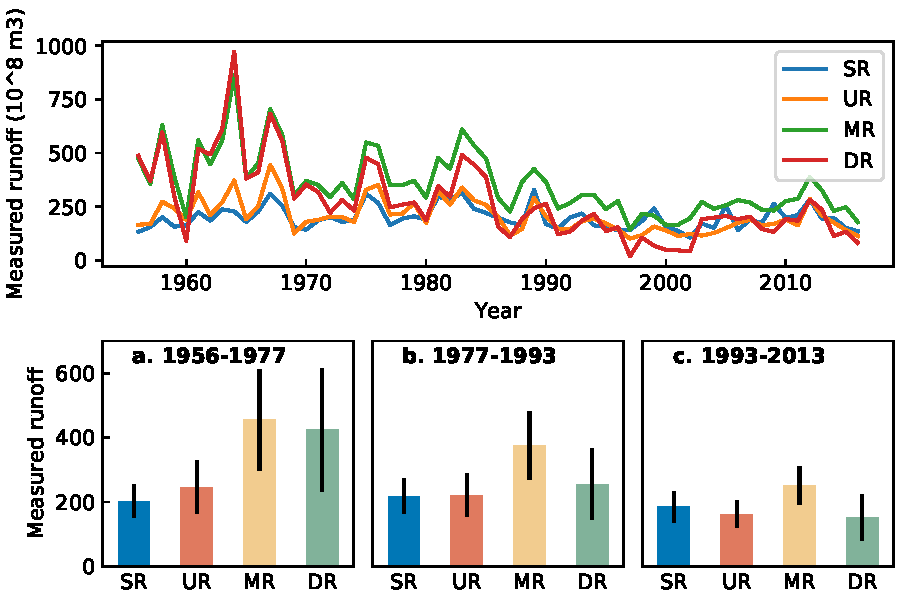
\includegraphics[width=\textwidth]{../../figures/supplementary_information/sf_measured_runoff.pdf}
\caption{Natural measured runoff of Yellow River within different periods.}
\end{figure}

\begin{figure}
\centering
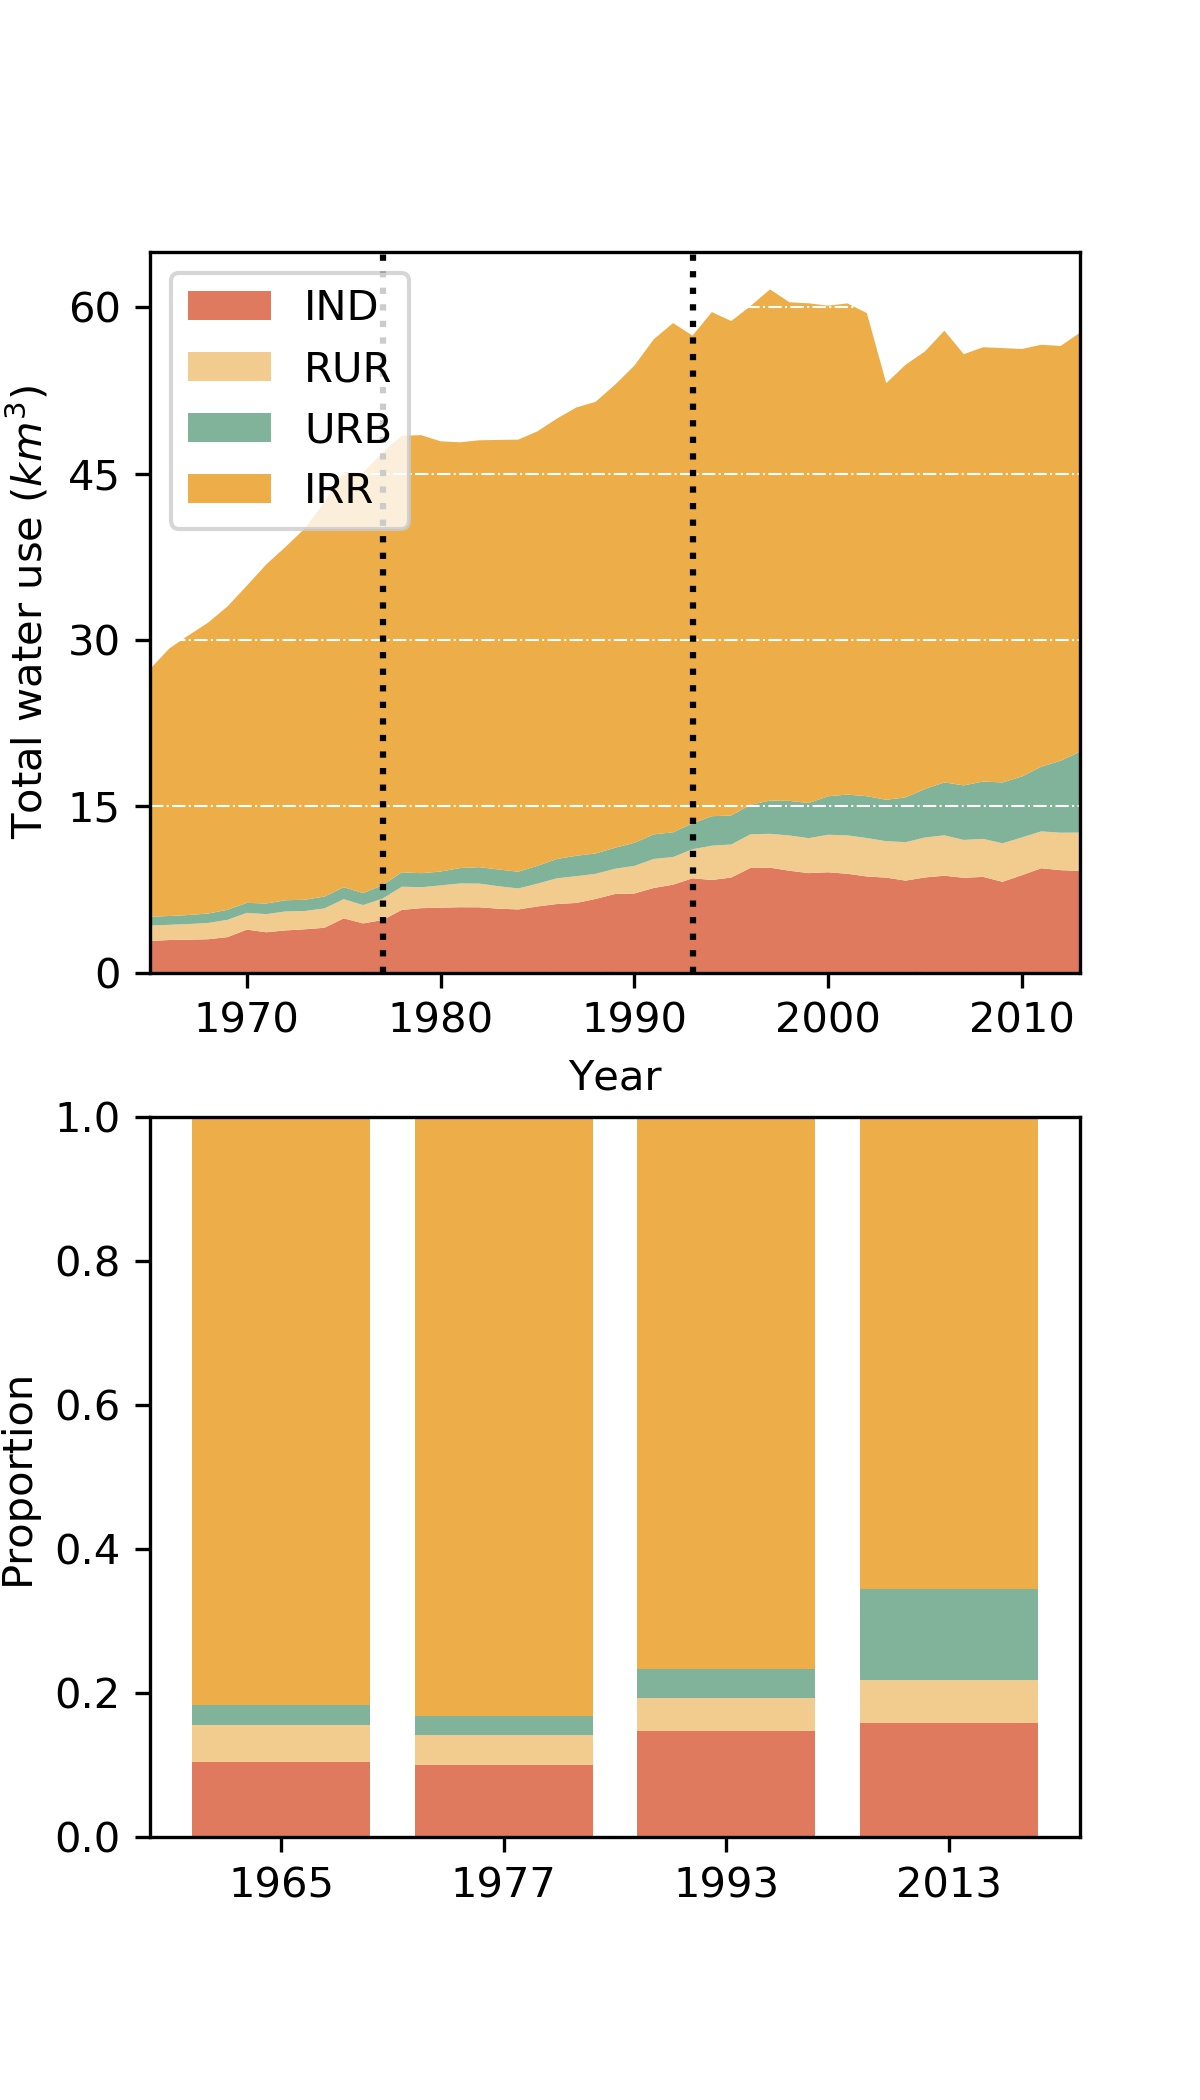
\includegraphics[width=\textwidth]{../../figures/supplementary_information/sf_wu_sections_stackplot.jpg}
\caption{Second figure}
\end{figure}

\begin{table}\centering
\caption{This is a table}

% 表格
\begin{tabular}{lrrr}
Species & CBS & CV & G3 \\
\midrule
1. Acetaldehyde & 0.0 & 0.0 & 0.0 \\
2. Vinyl alcohol & 9.1 & 9.6 & 13.5 \\
3. Hydroxyethylidene & 50.8 & 51.2 & 54.0\\
\bottomrule
\end{tabular}
\end{table}




%%% Add this line AFTER all your figures and tables
\FloatBarrier

\dataset{dataset_one.txt}{Type or paste legend here.}

\dataset{dataset_two.txt}{Type or paste legend here. Adding longer text to show what happens, to decide on alignment and/or indentations for multi-line or paragraph captions.}

\bibliography{pnas-sample}

\end{document}